\documentclass{scrartcl}
\title{\rmfamily Software Engineering -- Blatt 3}
\author{Rasmus Diederichsen \and Felix Breuninger\and % ugly hack, why does \\ ... work no more?
   \texttt{\{rdiederichse, fbreunin\}@uos.de}
}
\date{\today}
\usepackage[ngerman]{babel}
\usepackage[table]{xcolor}
\usepackage{arydshln}
\usepackage{microtype,
   textcomp,
   xifthen,
   multirow,
   booktabs,
   dingbat,
   titlesec,
   enumitem,
   fullpage,
   tikz,
   IEEEtrantools,
   array,
   amsmath,
   amssymb,
   graphicx,
   subcaption,
lmodern}
\usepackage[pdftitle={Software Engineering -- Blatt 3}, 
   pdfauthor={Rasmus Diederichsen}, 
   hyperfootnotes=true,
   colorlinks,
   bookmarksnumbered = true,
   linkcolor = lightgray,
   plainpages = false,
citecolor = lightgray]{hyperref}
\usepackage[utf8]{inputenc}
\usepackage[T1]{fontenc}
\usepackage[all]{hypcap}
% \renewcommand{\subsection}[1]{\noindent\bf Aufgabe \arabic{section}.\arabic{subsection}: #1}
\titleformat{\subsection}[hang]{\bf}{Aufgabe \arabic{section}.\arabic{subsection}:}{1em}{}[]
\titleformat{\subsubsection}[hang]{\bf}{\hspace{1em}\alph{subsubsection})}{1em}{}[]


\begin{document}

\fontfamily{ptm}\selectfont
\maketitle


\setcounter{section}{3}
\setcounter{subsection}{0}
\subsection{Projektstrukturplan (20 Punkte)}

Wir wählen einen phasenorientierten PSP. Dies bietet sich an, da der Aufgabentext
diese schon explizit vorgibt, was uns deshalb Arbeit erspart.\leftthumbsup

\usetikzlibrary{trees,calc}
\begin{center}
   \begin{tikzpicture}[
         work package/.style={draw,rectangle,text width=3cm},
         phase/.style={fill=gray!20,rounded corners=5pt,line width=1pt,text centered,font=\bf},
         grandchild/.style={grow=down,
         edge from parent path={(\tikzparentnode.west) -- ++(-1em,0) |- ($(\tikzparentnode.south west) + (-1em,0)$) |- (\tikzchildnode.west)}},
         first/.style={level distance=6ex},
         second/.style={level distance=14ex},
         third/.style={level distance=22ex},
         fourth/.style={level distance=30ex},
         fifth/.style={level distance=38ex},
         sixth/.style={level distance=46ex},
         seventh/.style={level distance=54ex},
         eighth/.style={level distance=62ex},
         level 1/.style={sibling distance=4cm,level distance=2cm}
      ]
      % \foreach \x / \y in {first/1,second/2,third/3,fourth/4,fifth/5,sixth/6,seventh/7,eight/8,ninth/9}
      % {\tikzstyle{\x}=[level distance=\pgfmathparse{\y * 6}\pgfmathresult em]};
      % Parents
      \coordinate
      node[fill=blue!10,font=\bf,text width=6cm,draw,text centered] {Client-Server-System für Versicherung}
      % child[grow=left] {node[work package,anchor=east]{Jim}}
      % child[grow=right] {node[work package,anchor=west]{Jane}}
      % child[grow=down,level distance=0ex]
      [edge from parent fork down]
      % Children and grandchildren
      child{node[work package,phase] {Phase 1}
         child[grandchild,first] {node[work package] {\textbf{A:} Funktionen erarbeiten}}
         child[grandchild,second] {node[work package] {\textbf{B:} Funktionen einteilen}}
         child[grandchild,third] {node[work package] {\textbf{C:} Schnittstellen zu Fremdsystemen}}
         child[grandchild,fourth] {node[work package] {\textbf{D:} Datenbankentwurf}}
         child[grandchild,fifth] {node[work package] {\textbf{E:} GUI-Prototyp entwickeln}}
      }
      child{node[work package,phase] {Phase 2}
         child[grandchild,first] {node[work package] {\textbf{F:} DB-Migration}}
         child[grandchild,second] {node[work package] {\textbf{G:} DB-Test}}
         child[grandchild,third] {node[work package] {\textbf{H:} Schnittstellen zu Fremdsystemen}}
         child[grandchild,fourth] {node[work package] {\textbf{I:} Clientimplementierung}}
         child[grandchild,fifth] {node[work package] {\textbf{J:}
         Server-DB-Integration}}
         child[grandchild,sixth] {node[work package] {\textbf{K:} Client-Server-Integration}}
         child[grandchild,seventh] {node[work package] {\textbf{L:} 1. Systemtest}}
      }
      child{node[work package,phase] {Phase 3}
         child[grandchild,first] {node[work package] {\textbf{M:} Serverfunkt. überarbeiten}}
         child[grandchild,second] {node[work package] {\textbf{N:} Ausbaufunktion.  implementieren}}
         child[grandchild,third] {node[work package] {\textbf{O:} GUI-Fehler beheben}}
         child[grandchild,fourth] {node[work package] {\textbf{P:} GUI für Ausbaufunkt. implementieren}}
         child[grandchild,fifth] {node[work package] {\textbf{Q:} Vollt. Datenmigration}}
         child[grandchild,sixth] {node[work package] {\textbf{R:} Integration Ausbaufunkt.  und Ausbau-GUI}}
         child[grandchild,seventh] {node[work package] {\textbf{S:} 2. Systemtest (Testfiliale)}}
         child[grandchild,eighth] {node[work package] {\textbf{T:} 2. Systemtest (Testteam)}}
      }
      child{node[work package,phase] {Phase 4}
         child[grandchild,first] {node[work package] {\textbf{U:} Korrektur/Optimierung}}
         child[grandchild,second] {node[work package] {\textbf{V:} Doku/Handbuch}}
         child[grandchild,third] {node[work package] {\textbf{W:} Schulung}}
         child[grandchild,fourth] {node[work package] {\textbf{X:} Deployment}}
      };

   \end{tikzpicture}

\end{center}
\subsection{Vorgangsliste (15 Punkte)}
\begin{center}
   \rowcolors{2}{gray!10}{white}
   \renewcommand{\arraystretch}{1.5}
   \begin{tabular}{l:lllr}
      \toprule
      &Bezeichner & Arbeitspaket & Abhängigkeiten & Dauer\\
      \midrule
      \cellcolor{white}&A & Funktionen erarbeiten & & 2W\\
      \cellcolor{white}&B & Funktionen einteilen & A & 1W\\
      \cellcolor{white}&C & Schnittstellen zu Fremdsystemen & A & 1W\\
      \cellcolor{white}&D & Datenbankentwurf & & 2W \\
      \cellcolor{white}\multirow{-5}{*}{\rotatebox[origin=c]{90}{Phase 1}}
      &E & GUI-Prototyp entwickeln & A & 1.5W\\
      \midrule
      \cellcolor{white}&F & DB-Migration & D & 2W \\
      \cellcolor{white}&G & DB-Test & F& 1W \\
      \cellcolor{white}&H & Schnittstellen zu Fremdsystemen & F, B, C & 7W \\
      \cellcolor{white}&I & Clientimplementierung & E & 5W \\
      \cellcolor{white}&J & Server-DB-Intergation & H, G& 1W \\
      \cellcolor{white}&K & Client-Server-Integration & I, J & 1W \\
      \cellcolor{white}\multirow{-7}{*}{\rotatebox[origin=c]{90}{Phase 2}}&L & 1. Systemtest & K & 1W \\
      \midrule
      \cellcolor{white}&M & Serverfunkt. überarbeiten & L, H, J& 2W \\
      \cellcolor{white}&N & Ausbaufunktion.  implementieren & B & 4W\\
      \cellcolor{white}&O & GUI-Fehler beheben & E, K & 1W \\
      \cellcolor{white}&P & GUI für Ausbaufunkt. implementieren & H & 2W \\
      \cellcolor{white}&Q & Vollt. Datenmigration & G & 2W \\
      \cellcolor{white}&R & Integration Ausbaufunkt.  und Ausbau-GUI & P, N, M, O & 2W \\
      \cellcolor{white}&S & 2. Systemtest (Testfiliale) & R, Q & 1W \\
      \cellcolor{white}\multirow{-8}{*}{\rotatebox[origin=c]{90}{Phase 3}}&T & 2. Systemtest (Testteam) & R, Q & 1W \\
      \midrule
      \cellcolor{white}&U & Korrektur/Optimierung & S, T & 2W \\
      \cellcolor{white}&V & Doku/Handbuch & U & 2W \\
      \cellcolor{white}&W & Schulung & U, V & 2W \\
      \cellcolor{white}\multirow{-4}{*}{\rotatebox[origin=c]{90}{Phase 4}}&X & Deployment &  V, W & 4W\\
      \bottomrule
   \end{tabular}
\end{center}
\subsection{Netzplan (25 Punkte)}

\usetikzlibrary{positioning,matrix}
% This is for the outer glow. Taken from
% http://tex.stackexchange.com/questions/42810/can-i-have-a-glow-around-a-box-in-tikz
\def\shadowradius{3pt}
%
\newcommand\drawshadowbis[1]{
    \begin{pgfonlayer}{shadow}
        \fill[inner color=red,outer color=white] ($(#1.south west)$) circle (\shadowradius);
        \fill[inner color=red,outer color=white] ($(#1.north west)$) circle (\shadowradius);
        \fill[inner color=red,outer color=white] ($(#1.south east)$) circle (\shadowradius);
        \fill[inner color=red,outer color=white] ($(#1.north east)$) circle (\shadowradius);
        \fill[top color=red,bottom color=white] ($(#1.south west)+((0,-\shadowradius)$) rectangle ($(#1.south east)$);
        \fill[left color=red,right color=white] ($(#1.south east)$) rectangle ($(#1.north east)+((\shadowradius,0)$);
        \fill[bottom color=red,top color=white] ($(#1.north west)$) rectangle ($(#1.north east)+((0,\shadowradius)$);
        \fill[right color=red,left color=white] ($(#1.south west)$) rectangle ($(#1.north west)+(-\shadowradius,0)$);
\end{pgfonlayer}
}
%
\pgfdeclarelayer{shadow} 
\pgfsetlayers{shadow,main}

\tikzstyle{cell}=[minimum height=1.5em,anchor=west,draw,text centered,text width=1.5em]
\newcommand{\boxnode}[5]{% \boxnode{name}{earliest start}{duration}{latest end}{pos cmds}
   \matrix[
      #5,
      matrix of nodes,
      nodes={cell},
      inner sep=0pt,
      outer sep=0pt,
      ampersand replacement=\&,
      row sep=-.5pt,
      column sep=-.5pt,
      nodes={font=\small},
      row 1/.style={nodes={fill=white,draw=none}},
      row 2/.style={nodes={fill=gray!10}},
      row 3/.style={nodes={fill=gray!30}},
   ] (#1) {
      {} \& #1 \& {}\\ % pgfmathparse parses the expression, pgfmathprintnumber is for ommitting the fractional part
      #2\& #3 \& \pgfmathparse{#2+#3}\pgfmathprintnumber{\pgfmathresult}\\
      \pgfmathparse{#4-#3}\pgfmathprintnumber{\pgfmathresult}\& \pgfmathparse{#4-#3-#2}\pgfmathprintnumber{\pgfmathresult} \& #4 \\
   };
   \draw (#1-1-1.south west) -- (#1-1-1.north west) -- (#1-1-3.north east) -- (#1-1-3.south east);
   \pgfmathparse{int(#4-#3-#2)}
   \ifnum\pgfmathresult=0
      \drawshadowbis{#1}
   \fi
}
\usetikzlibrary{arrows}
\tikzset{
arrow/.style={-latex, shorten >=1ex, shorten <=1ex}}

Legende:

\begin{center}
      \begin{tikzpicture}[transform canvas={scale=0.6}]
         \boxnode{A}{0}{2}{5}{}
         \node[left=of A.west] (start) {Frühester Beginn};
         \node[below=of start] (start_late) {Spätester Beginn};
         \node[below=of A.south] (puffer) {Puffer};
         \node[right=of A.east] (end) {Frühestes Ende};
         \node[below=of end] (end_late) {Spätestes Ende};
         \node[above=of A] (bez) {Bezeichner};
         \node[right=of bez] (dauer) {Dauer};

         \draw[arrow, bend left,bend angle=45] (start) to (A.west);
         \draw[arrow, bend right,bend angle=45] (start_late) to (A.south west);
         \draw[arrow,,shorten >=5pt] (puffer) -- (A.south);
         \draw[arrow, bend left,bend angle=45] (end_late) to (A.south east);
         \draw[arrow, bend right,bend angle=45] (end) to (A.east);
         \draw[arrow,,shorten >=8pt] (dauer) -- (A.center);
         \draw[arrow, bend left,bend angle=45] (bez) to (A.north);
      \end{tikzpicture}
\end{center}

\begin{center}
   \begin{tikzpicture}[node distance=1.5cm]
      \boxnode{A}{0}{2}{3}{}
      \boxnode{B}{2}{1}{4}{right=of A}
      \boxnode{C}{2}{1}{4}{below=of B}
      \boxnode{D}{0}{2}{2}{below=of A}
      \boxnode{E}{2}{1.5}{7}{below=of C}

      \boxnode{F}{2}{2}{4}{right=of B}
      \boxnode{G}{4}{1}{11}{right=of F}
      \boxnode{H}{4}{7}{11}{below=of F}
      \boxnode{I}{3.5}{5}{12}{below=of H}
      \boxnode{J}{11}{1}{12}{right=of H}
      \boxnode{K}{12}{1}{13}{below=of J}
      \boxnode{L}{13}{1}{14}{right=of J}

      \boxnode{M}{14}{2}{16}{below left=2cm and 1cm of E}
      \boxnode{N}{3}{4}{16}{right=of M}
      \boxnode{O}{13}{1}{16}{right=of N}
      \boxnode{Q}{5}{2}{17}{right=of O}
      \boxnode{R}{16}{2}{18}{below=of M}
      \boxnode{P}{11}{2}{16}{right=of R}
      \boxnode{S}{18}{1}{19}{right=of P}

      \boxnode{T}{18}{1}{19}{below=2cm of R}
      \boxnode{U}{19}{2}{21}{right=of T}
      \boxnode{V}{21}{2}{23}{right=of U}
      \boxnode{W}{23}{2}{25}{right=of V}
      \boxnode{X}{25}{2}{27}{right=of W}

      \draw[thick,->] (A.east) -- ($(A.east) + (1em,0em)$) -- (B.west);
      \draw[thick,->] ($(A.east) + (1em,0em)$) |- (C.west);
      \draw[thick,->] ($(A.east) + (1em,0em)$) |- (E.west);
      \draw[thick,->] (D.north) |- ($(F.south) + (-.5em,-1em)$) -| ($(F.south) + (-.5em,0em)$);
      \draw[thick,->] (C.east) -- (H.west);
      \draw[thick,-] (B.east) -| ($(H.west) + (-1em,0em)$);
      \draw[thick,->] ($(B.west) + (0em,-1em)$) -- ++(-1em,0em) |- ($(N.west) + (-1em,0em)$) -- (N.west);
      \draw[thick,->] (F.south) -- (H.north);
      \draw[thick,->] (F.east) -- (G.west);
      \draw[thick,->] (H.east) -- (J.west);
      \draw[thick,->] (E.east) -- (I.west);
      \draw[thick,->] (I.east) -- (K.west);
      \draw[thick,->] (K.east) -| ($(L.west) + (-1em,0em)$) |- (L.west);
      \draw[thick,->] (J.south) -- (K.north);
      \draw[thick,->] (G.south) -- (J.north);
      \draw[thick,->] (E.south) |- ($(O.north) + (0em,1em)$) -- (O);
      \draw[thick,-] (K.south) |- ($(O.north) + (0em,1em)$);
      % \draw[thick,->] (B.east) -| ($(N.east) + (1em,0em)$) -- (N.east);
      \draw[thick,-] ($(J.east) + (0em,-1em)$) -| ($(J.east) + (1em,-13em)$) -| (M.north);
      \draw[thick,-] ($(H.east) + (0em,-1em)$) -| ($(H.east) + (1em,-13em)$) -| (M.north);
      \draw[thick,->] ($(L.east) + (0em,-1em)$) -| ($(L.east) + (1em,-13em)$) -| (M.north);
      \draw[thick,->] ($(H.west) + (0em,-.5em)$) -| ($(P.east) + (1.5em,.5em)$) -- ($(P.east) + (0em,.5em)$);
      \draw[thick,->] (G.east) -| ++(10em,-20em) |- (Q.east);
      % \draw[thick,->] (N.south) |- ($(P.north) + (0em,1em)$) -- (P);
      % \draw[thick,-] (O.south) |- ($(P.north) + (0em,1em)$);
      \draw[thick,-] ($(O.south) + (-1em,0em)$) |- ($(R.north) + (0em,1em)$);
      \draw[thick,->] (M.south) -- (R);
      \draw[thick,-] ($(N.south) + (-1em,0em)$) |- ($(R.north) + (0em,1em)$);
      \draw[thick,-] (P.west) -- ++(-1em,0em) |- ($(R.north) + (0em,1em)$);
      \draw[thick,->] (Q.south) |- (S.east);
      \draw[thick,->] ($(R.south) + (1em,0em)$) -- ++(0em,-1em) -| ($(S.south) + (-1em,0em)$);
      \draw[thick,->] (R.south) -- (T.north);
      \draw[thick,-] ($(Q.south) + (1em,0em)$) |- ($(T.north) + (0em,3em)$);
      \draw[thick,->] (T.east) -- (U.west);
      \draw[thick,->] (U.east) -- (V.west);
      \draw[thick,-] ($(U.north) + (1em,0em)$) -- ++(0em,.5em) -| ($(W.west) + (-1em,0em)$);
      \draw[thick,->] (S.west) -| ($(U.east) + (1em,1em)$) -- ($(U.east) + (0em,1em)$);
      \draw[thick,->] (V.east) -- (W.west);
      \draw[thick,-] ($(V.south) + (1em,0em)$) -- ++(0em,-.5em) -| ($(X.west) + (-1em,0em)$);
      \draw[thick,->] (W.east) -- (X.west);
   \end{tikzpicture}
\end{center}
\subsection{Gantt-Diagramm (20 Punkte)}

 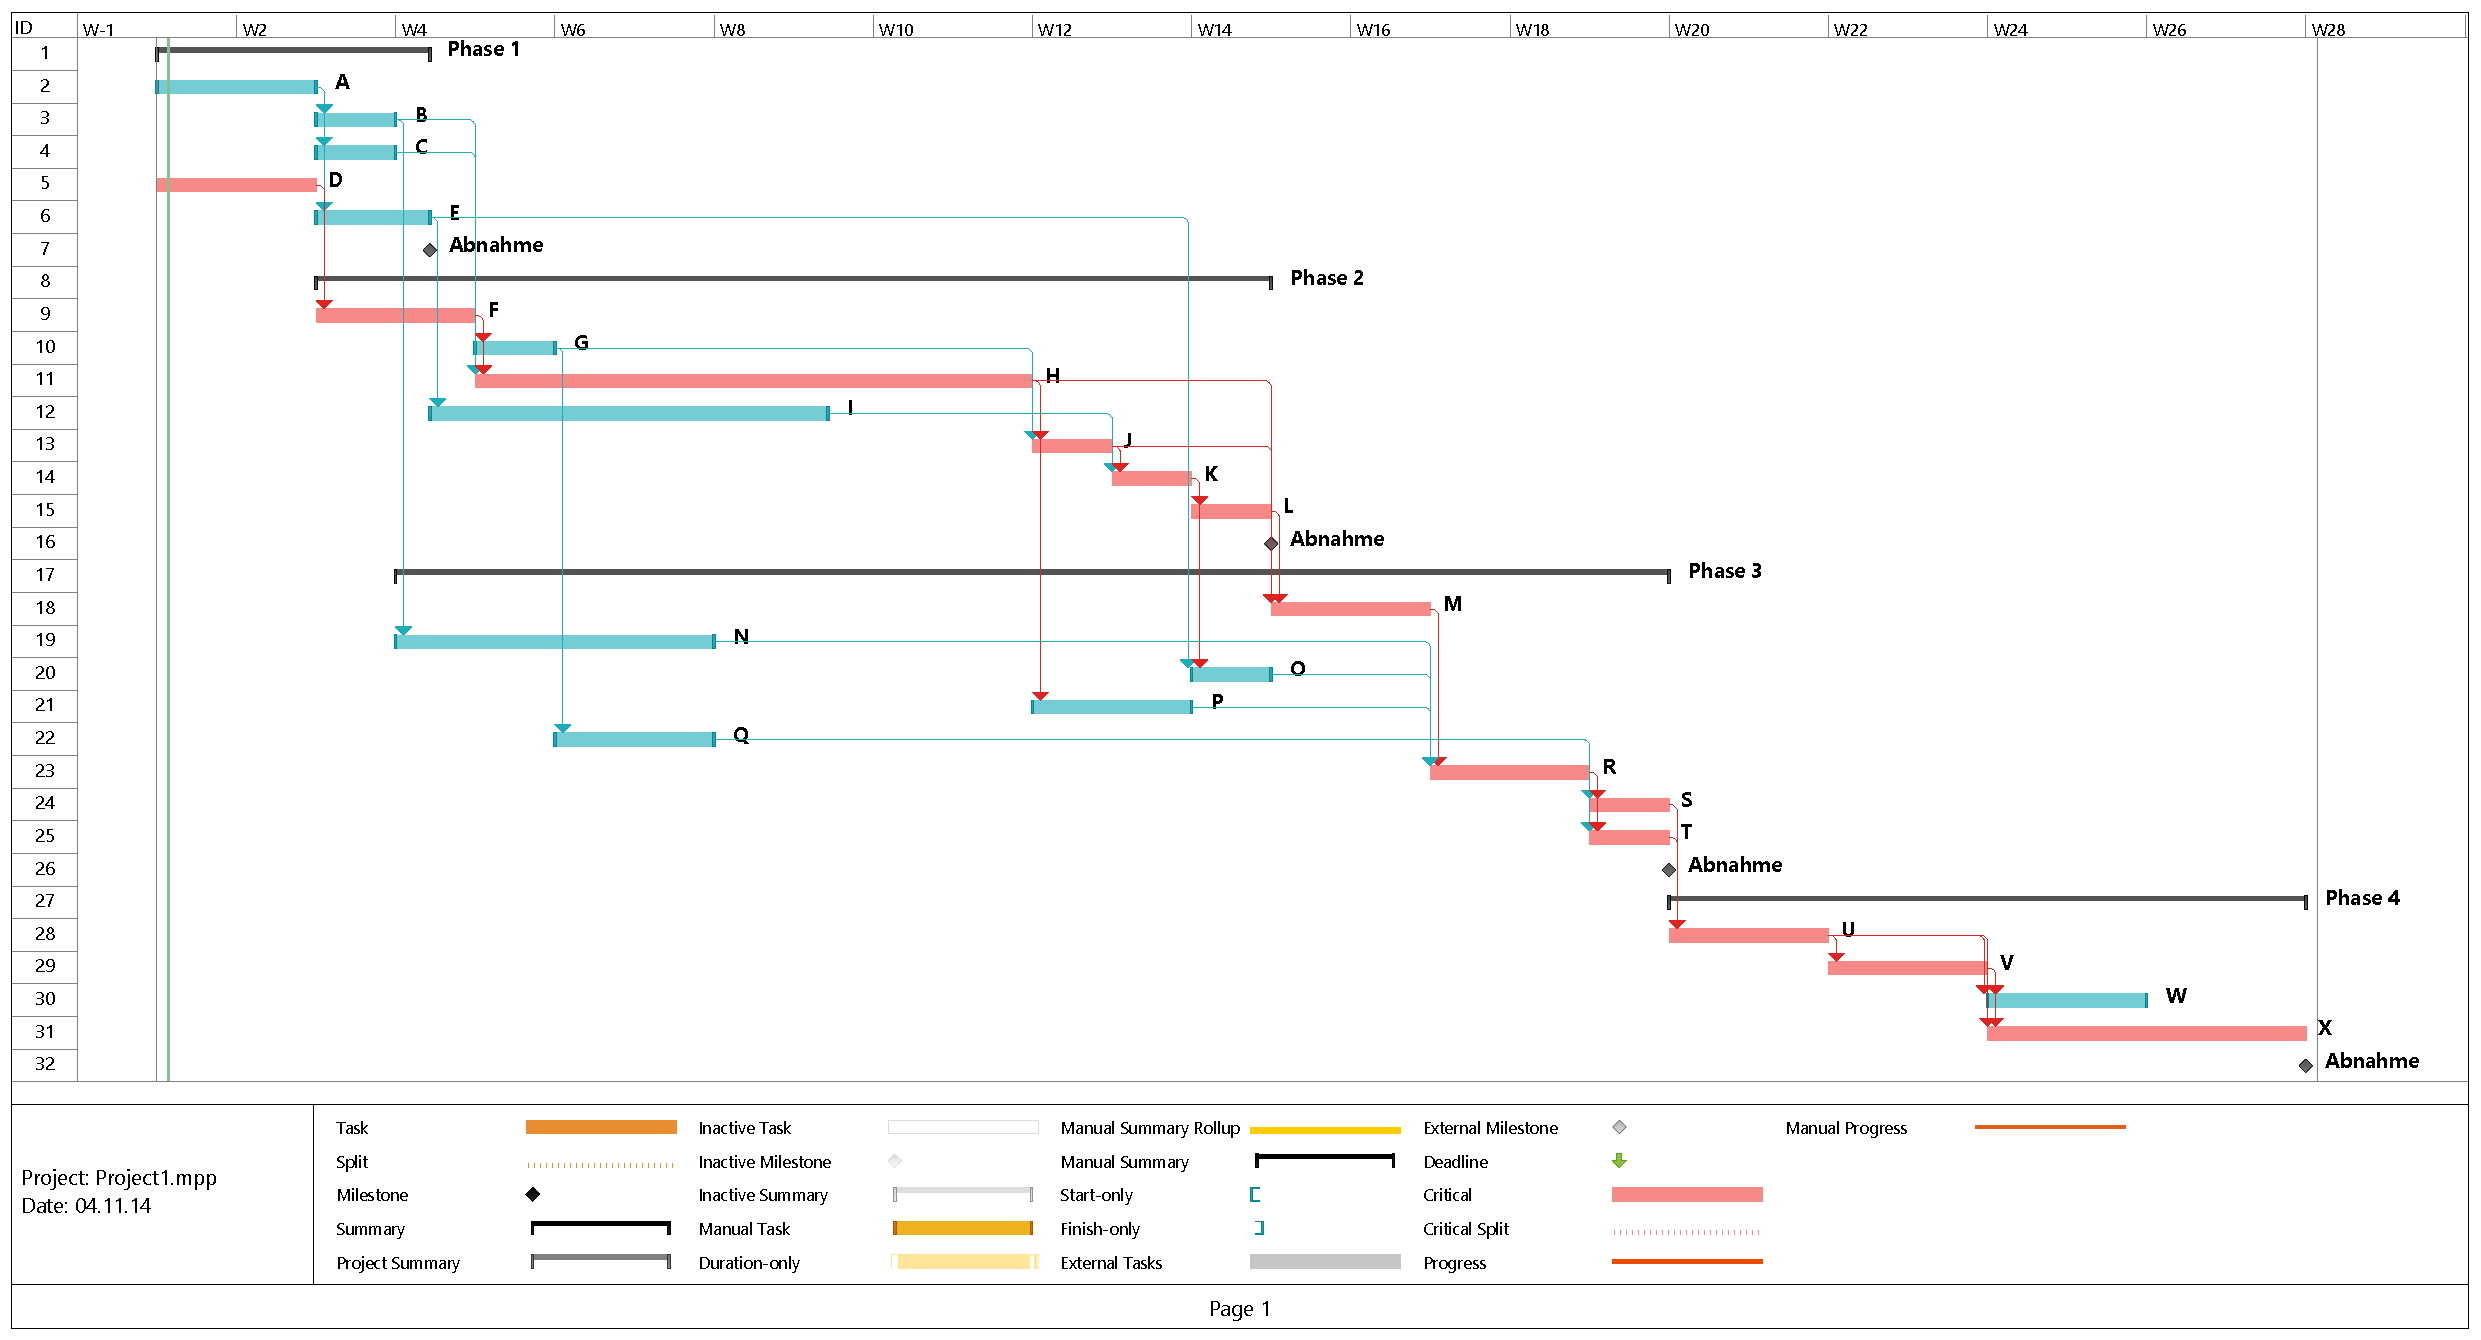
\includegraphics[width=\linewidth]{gantt.pdf}


\subsection{Firmenorganisation (10 Punkte)}
\subsubsection*{Firmenorganisation}

Im Bezug auf die Gesamtorganisation der Firma wäre eine funktionale Organisation
durchaus sinnig, da viele Mitarbeiter vorhanden sind, die an vielen
verschiedenen Baustellen arbeiten, welche unterschiedliche Spezialisten
benötigen (UX-Designer, Datenbankexperte, Servertechniker etc). Diese
Spezialisten lassen sich dann auch in verschiedene Abteilungen einteilen. Da bei den
vielen Arbeitspaketen jedoch unterschiedliche Kombinationen dieser Spezialisten
zwecks Integration nötig sind, bieten sich orthogonal dazu temporäre
Entwicklerteams an, was zu einer Matrixorganisation führt.

\subsubsection*{Teamorganisation}
Bei kleineren Projekten bietet es
sich an, Chief-Programmer-Teams zur Umsetzung einzusetzen. Diese vereinen die
Stärken von hierarchischen und demokratischen Teams und gewährleisten somit
kurze Kommunikationswege in Kombination mit einer kollaborativen aber dennoch
strukturierten Projektumsetzung.

Für große Projekte lässt sich eine gewisse hierarchische Anordnung nicht
vermeiden, empfehlenswert ist also eine Mixed Control-Organisation. Diese ist
auch in großen Teams umsetzbar und verwendet hierarchische Strukturen zwischen
den Hierarchie-Ebenen, wohingegen innerhalb einer Hierarchie-Ebene demokratische
Strukturen eingesetzt werden und somit erneut die Vor- und Nachteile in
sinnvollem Verhältnis zueinander stehen.

\end{document}
